\documentclass{article}
\usepackage{graphicx}
\usepackage{subfigure}
\usepackage{float}
\usepackage[margin=1in]{geometry}
\usepackage{longtable}
\usepackage{booktabs}
\usepackage{array}
\usepackage{amsmath}
\usepackage{hyperref}
\usepackage{xurl}
\usepackage[backend=biber,style=numeric]{biblatex}
\addbibresource{references.bib}

\hypersetup{
  colorlinks = true,
  urlcolor   = blue,
  citecolor  = blue,
  breaklinks = true
}

\newcolumntype{P}[1]{>{\raggedright\arraybackslash}p{#1}}

\title{Shadow Sinus}
\author{David Messner}
\date{June 2026}

\begin{document}
\maketitle\maketitle
\tableofcontents
\section{Hardware Used}
All training was performed on a local machine with the following
specifications:

\begin{itemize}
	\item \textbf{GPU:} NVIDIA GeForce RTX 3090 (24\,GB VRAM)
	\item \textbf{CPU:} Intel\textregistered\ Core\texttrademark\ i5-4570
	      (4 logical cores)
	\item \textbf{RAM:} 14.0\,GiB
	\item \textbf{Hardware Model:} HP EliteDesk 800 G1 TWR
	\item \textbf{OS:} Ubuntu 24.04.4 LTS
\end{itemize}

\section{Yolo}
You Only Look Once (YOLO) differs from earlier object detection models in
that it processes an image with a single neural network, rather than
splitting the task into two separate steps: first finding candidate boxes,
and then classifying what is inside them .

The first step the YOLO model performs is to divide the input image into a
grid. Each cell of this grid predicts a number of bounding boxes, and every
predicted box receives its own confidence score. This score combines two
things at once: whether the model believes an object is present in that
box, and how accurately it believes the box fits the object
. If no object is present in a given box, this
confidence value should be zero.

During training, these predicted values are compared against the
corresponding values computed from the ground-truth labels. The resulting
error is used to update the network's weights through gradient descent:
predictions that are already close to correct produce very little error
and are left largely unchanged, while predictions that are still wrong
produce a larger error and drive most of the learning. In this way, the
network gradually corrects only the parts of its output where it is
actually mistaken, rather than being adjusted uniformly across the whole
image.
\section{understanig yolo Modell graph}
\begin{figure}[H]
	\centering
	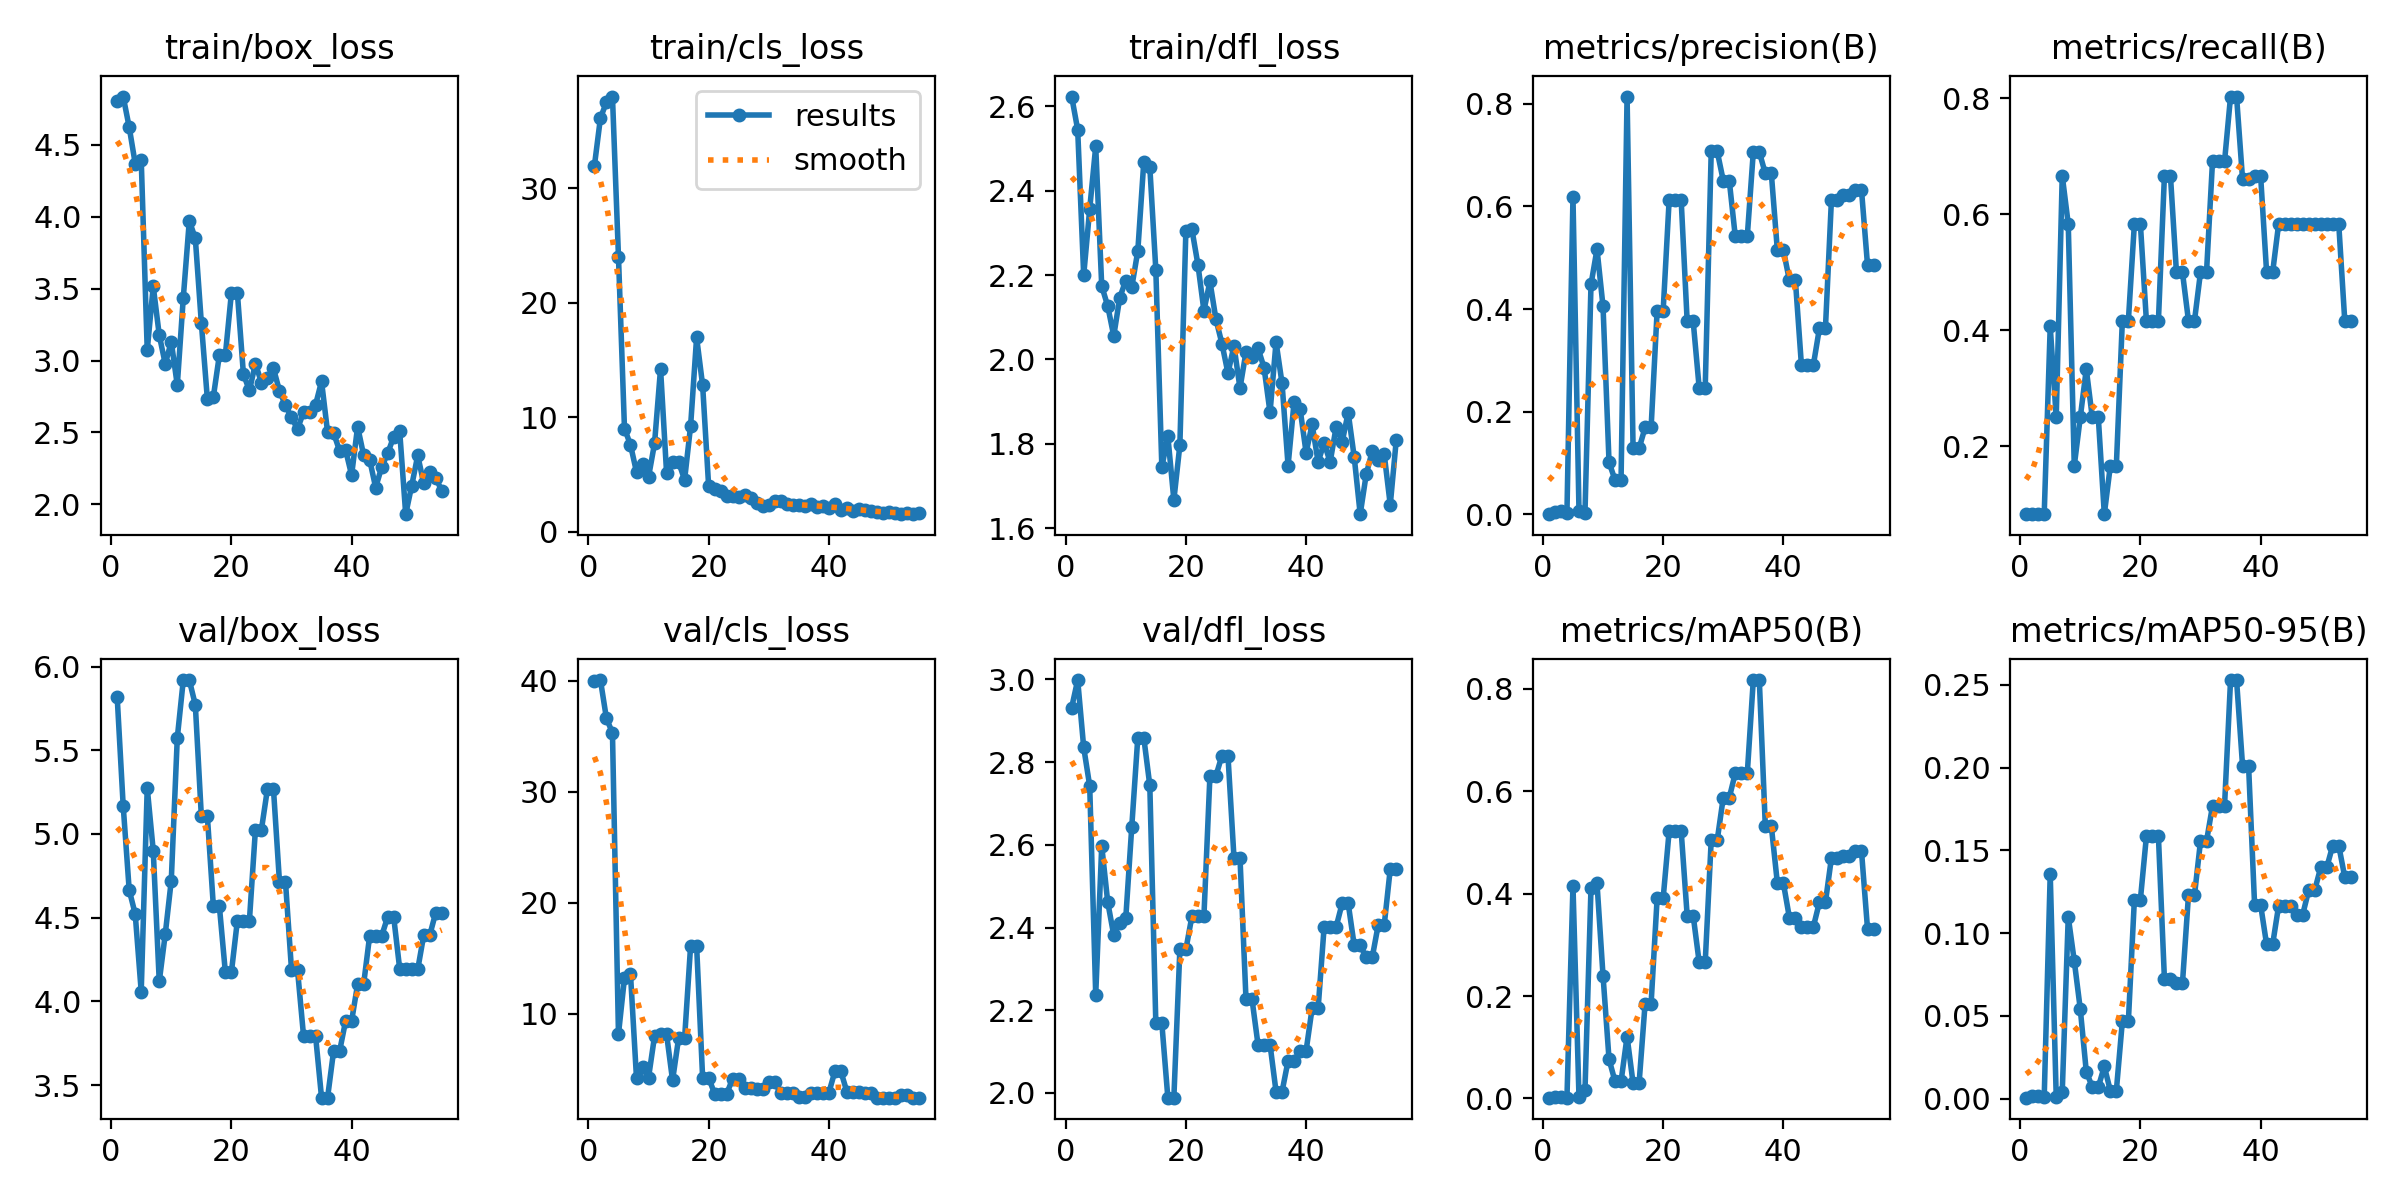
\includegraphics[width=1\linewidth]{pictures/train-1678/results.png}
	\caption{First test runs with each label: left side YOLOv8, right side YOLOv26.}
	\label{fig:result-graph}
\end{figure}
A standard YOLO performance visualization consists of ten distinct plots, each tracking a specific metric or loss component during the training process.\ref{fig:result-graph} As a general rule of thumb, any graph representing evaluation metrics should ideally display an upward trend, whereas plots representing loss functions should trend downward. Furthermore, a smooth, steady progression is preferable, as highly jagged curves typically indicate training instability or volatile learning steps.
\begin{itemize}
	\item \textbf{Box Loss:} Measures localization accuracy. A decreasing trend signifies that the model is learning to accurately place bounding boxes. If validation loss increases while training loss decreases, it suggests overfitting.
	\item \textbf{Class Loss:} Measures classification error. Rapid drops early in training indicate that the model is quickly learning to differentiate between categories. If validation class loss stays high, it suggests that the classes visually overlap.
	\item \textbf{Distribution Focal Loss (DFL):} Optimizes box edges by predicting probability distributions. A steady decrease indicates that the model is refining its boundaries to handle occlusions and blur. If the validation loss does not decrease, it suggests that the model is memorizing the training data rather than truly learning.
\end{itemize}

\section{Errors}
The total number of labels is 12, but that happens to be the value that is filtered out of 1000 images, so it is a label that does not occur often.

\section{Hypertune}
After some tests with hypertune, these were the best values that came out. If you look at the confusion matrix it showes even after Hypertuning and a value of 80. It showes that it makes mane mistakes and draws many boxes where there shouldn't be errros \ref{fig:confusion-matrix} The errors I can see that were made where just because the yolo modell made labeled some things 2 times.\ref{fig:results}, and I can't also not for the live of me find outh which one was worng in the labels. So the results are more promessing

\begin{verbatim}
"best_trial": 80,
 "best_mAP50": 0.8146015037593985,
 "best_params": {
   "hsv_v": 0.15995225034795865,
   "degrees": 0.13466208213948474,
   "translate": 0.09603134222692039,
   "scale": 0.19219535449476197,
   "shear": 9.736352052556036,
   "fliplr": 0.4141825966166511,
   "mosaic": 0.13776433872485452,
   "erasing": 0.3194174051547562,
   "lr0": 0.00017805444103867718,
   "lrf": 0.0011537012620618519,
   "cls": 0.8975067907692778,
   "box": 11.028296175840389
 },
\end{verbatim}
\begin{figure}[H]
	\centering
	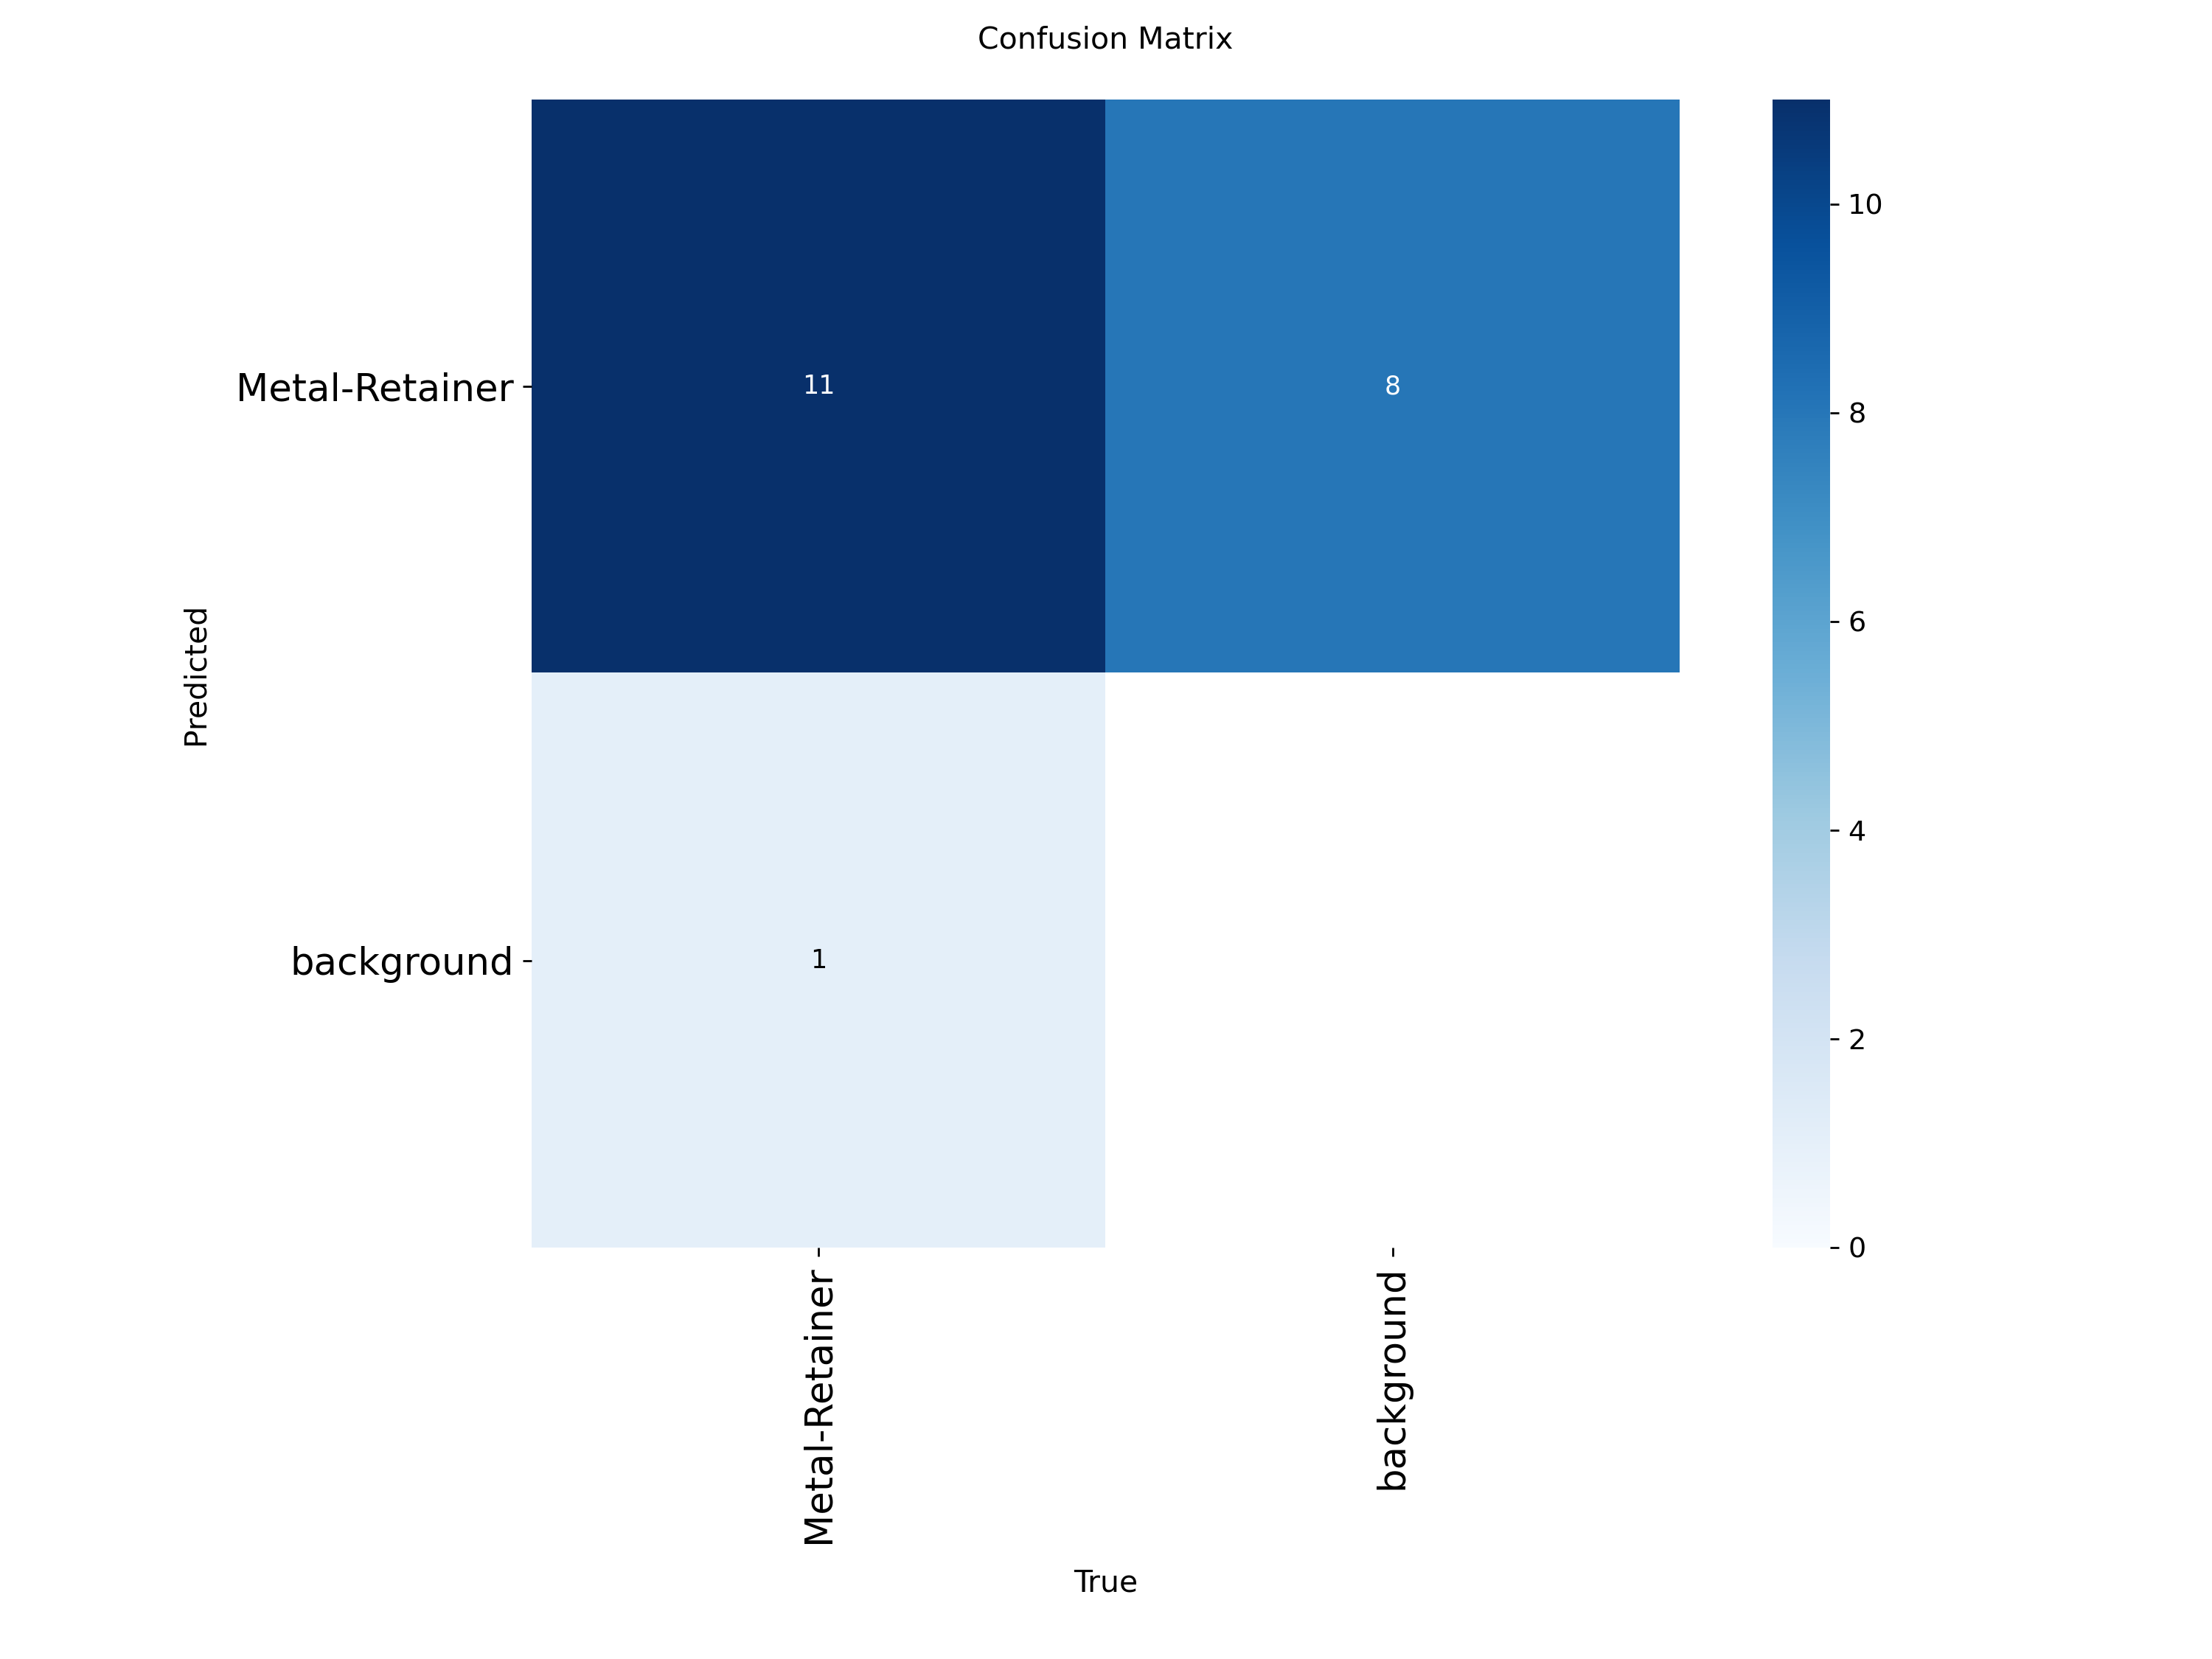
\includegraphics[width=1\linewidth]{pictures/train-1678/confusion_matrix.png}
	\caption{}
	\label{fig:confusion-matrix}
\end{figure}
\begin{figure}[H]
	\centering
	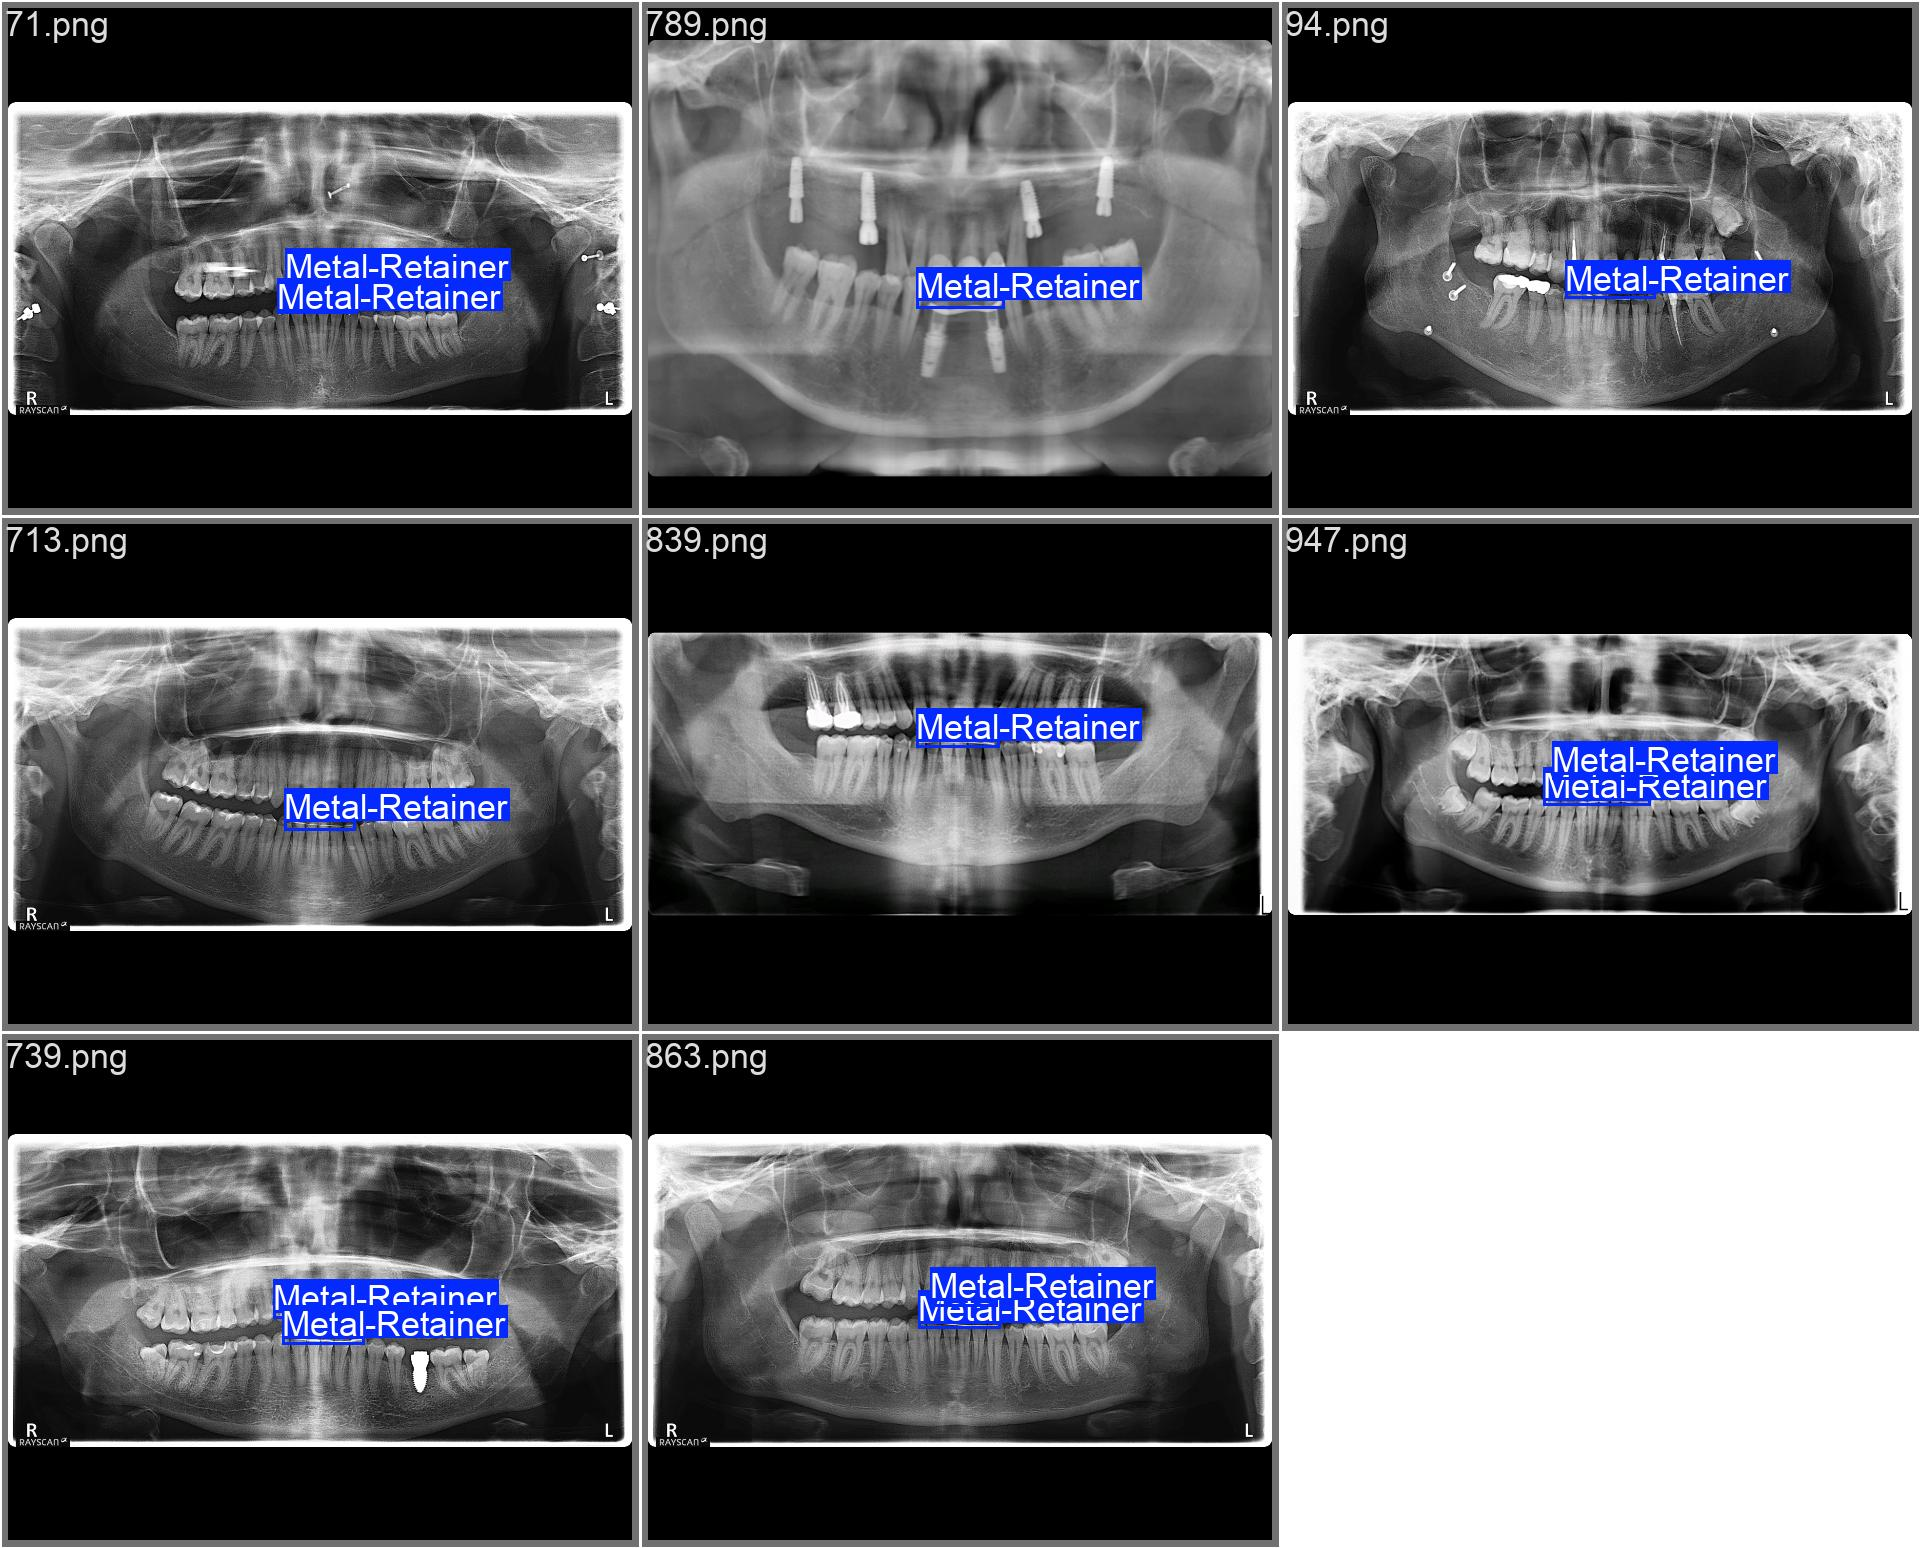
\includegraphics[width=0.48\linewidth]{pictures/train-1678/val_batch0_labels.jpg}%
	\hfill
	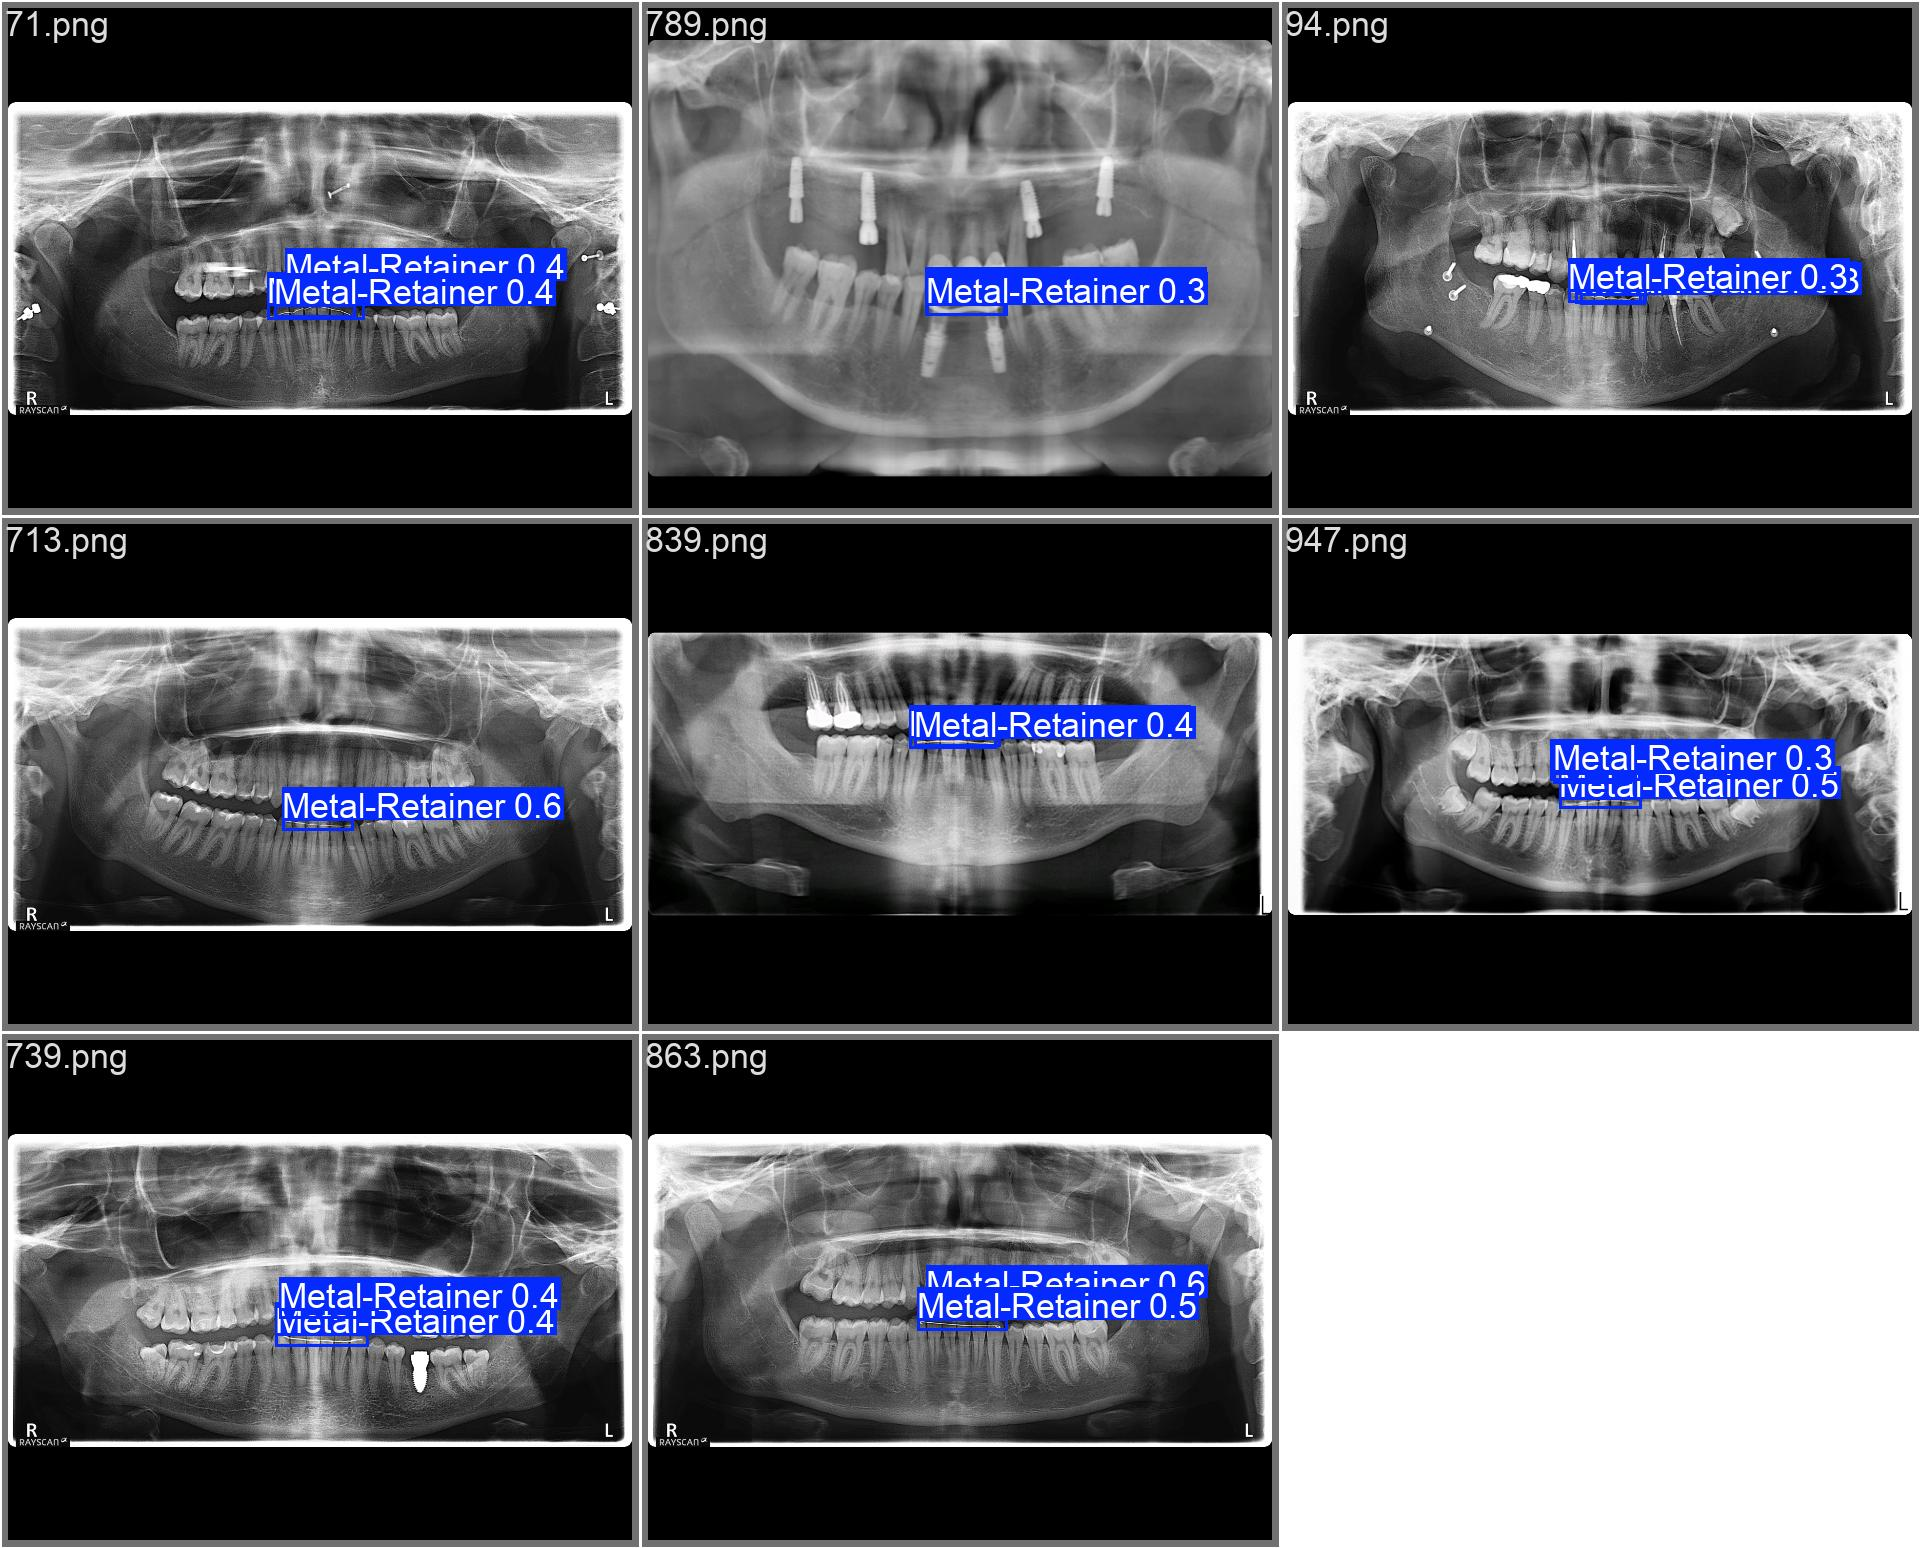
\includegraphics[width=0.48\linewidth]{pictures/train-1678/val_batch0_pred.jpg}
	\caption{Ground truth labels (left) and model predictions (right).}
	\label{fig:results}
\end{figure}
\end{document}
